% Options for packages loaded elsewhere
\PassOptionsToPackage{unicode}{hyperref}
\PassOptionsToPackage{hyphens}{url}
%
\documentclass[
  11pt,
]{article}
\usepackage[]{mathpazo}
\usepackage{amssymb,amsmath}
\usepackage{ifxetex,ifluatex}
\ifnum 0\ifxetex 1\fi\ifluatex 1\fi=0 % if pdftex
  \usepackage[T1]{fontenc}
  \usepackage[utf8]{inputenc}
  \usepackage{textcomp} % provide euro and other symbols
\else % if luatex or xetex
  \usepackage{unicode-math}
  \defaultfontfeatures{Scale=MatchLowercase}
  \defaultfontfeatures[\rmfamily]{Ligatures=TeX,Scale=1}
  \setmainfont[]{Palatino}
  \setsansfont[]{Helvetica Neue}
  \setmonofont[]{Monaco}
\fi
% Use upquote if available, for straight quotes in verbatim environments
\IfFileExists{upquote.sty}{\usepackage{upquote}}{}
\IfFileExists{microtype.sty}{% use microtype if available
  \usepackage[]{microtype}
  \UseMicrotypeSet[protrusion]{basicmath} % disable protrusion for tt fonts
}{}
\makeatletter
\@ifundefined{KOMAClassName}{% if non-KOMA class
  \IfFileExists{parskip.sty}{%
    \usepackage{parskip}
  }{% else
    \setlength{\parindent}{0pt}
    \setlength{\parskip}{6pt plus 2pt minus 1pt}}
}{% if KOMA class
  \KOMAoptions{parskip=half}}
\makeatother
\usepackage{xcolor}
\IfFileExists{xurl.sty}{\usepackage{xurl}}{} % add URL line breaks if available
\IfFileExists{bookmark.sty}{\usepackage{bookmark}}{\usepackage{hyperref}}
\hypersetup{
  hidelinks,
  pdfcreator={LaTeX via pandoc}}
\urlstyle{same} % disable monospaced font for URLs
\usepackage[margin=1in]{geometry}
\usepackage{graphicx,grffile}
\makeatletter
\def\maxwidth{\ifdim\Gin@nat@width>\linewidth\linewidth\else\Gin@nat@width\fi}
\def\maxheight{\ifdim\Gin@nat@height>\textheight\textheight\else\Gin@nat@height\fi}
\makeatother
% Scale images if necessary, so that they will not overflow the page
% margins by default, and it is still possible to overwrite the defaults
% using explicit options in \includegraphics[width, height, ...]{}
\setkeys{Gin}{width=\maxwidth,height=\maxheight,keepaspectratio}
% Set default figure placement to htbp
\makeatletter
\def\fps@figure{htbp}
\makeatother
\setlength{\emergencystretch}{3em} % prevent overfull lines
\providecommand{\tightlist}{%
  \setlength{\itemsep}{0pt}\setlength{\parskip}{0pt}}
\setcounter{secnumdepth}{-\maxdimen} % remove section numbering
\usepackage{fancyhdr} \setlength{\headheight}{14pt} \usepackage{soul} \usepackage{color} \usepackage{float} \usepackage{hyperref} \usepackage{sectsty} \sectionfont{\centering} \usepackage{enumitem} \usepackage{amsmath} \usepackage{amsfonts} \usepackage{bm} \usepackage{titling} \usepackage[hang,flushmargin]{footmisc} \usepackage{booktabs} \sectionfont{\bfseries\Large\raggedright}
\usepackage{booktabs}
\usepackage{longtable}
\usepackage{array}
\usepackage{multirow}
\usepackage{wrapfig}
\usepackage{float}
\usepackage{colortbl}
\usepackage{pdflscape}
\usepackage{tabu}
\usepackage{threeparttable}
\usepackage{threeparttablex}
\usepackage[normalem]{ulem}
\usepackage{makecell}
\usepackage{xcolor}

\title{\fontsize{15pt}{5pt}\selectfont\textbf{Final Examination}\\
\vspace{.3cm}\textbf{PB HLTH 250C: Advanced Epidemiologic Methods}\\
\vspace{.2cm}\textbf{Katherine Rose Wolf}\\
\vspace{.3cm}\textbf{\today}}
\author{}
\date{\vspace{-2.5em}}

\begin{document}
\maketitle

\pagestyle{plain}

\begin{center}

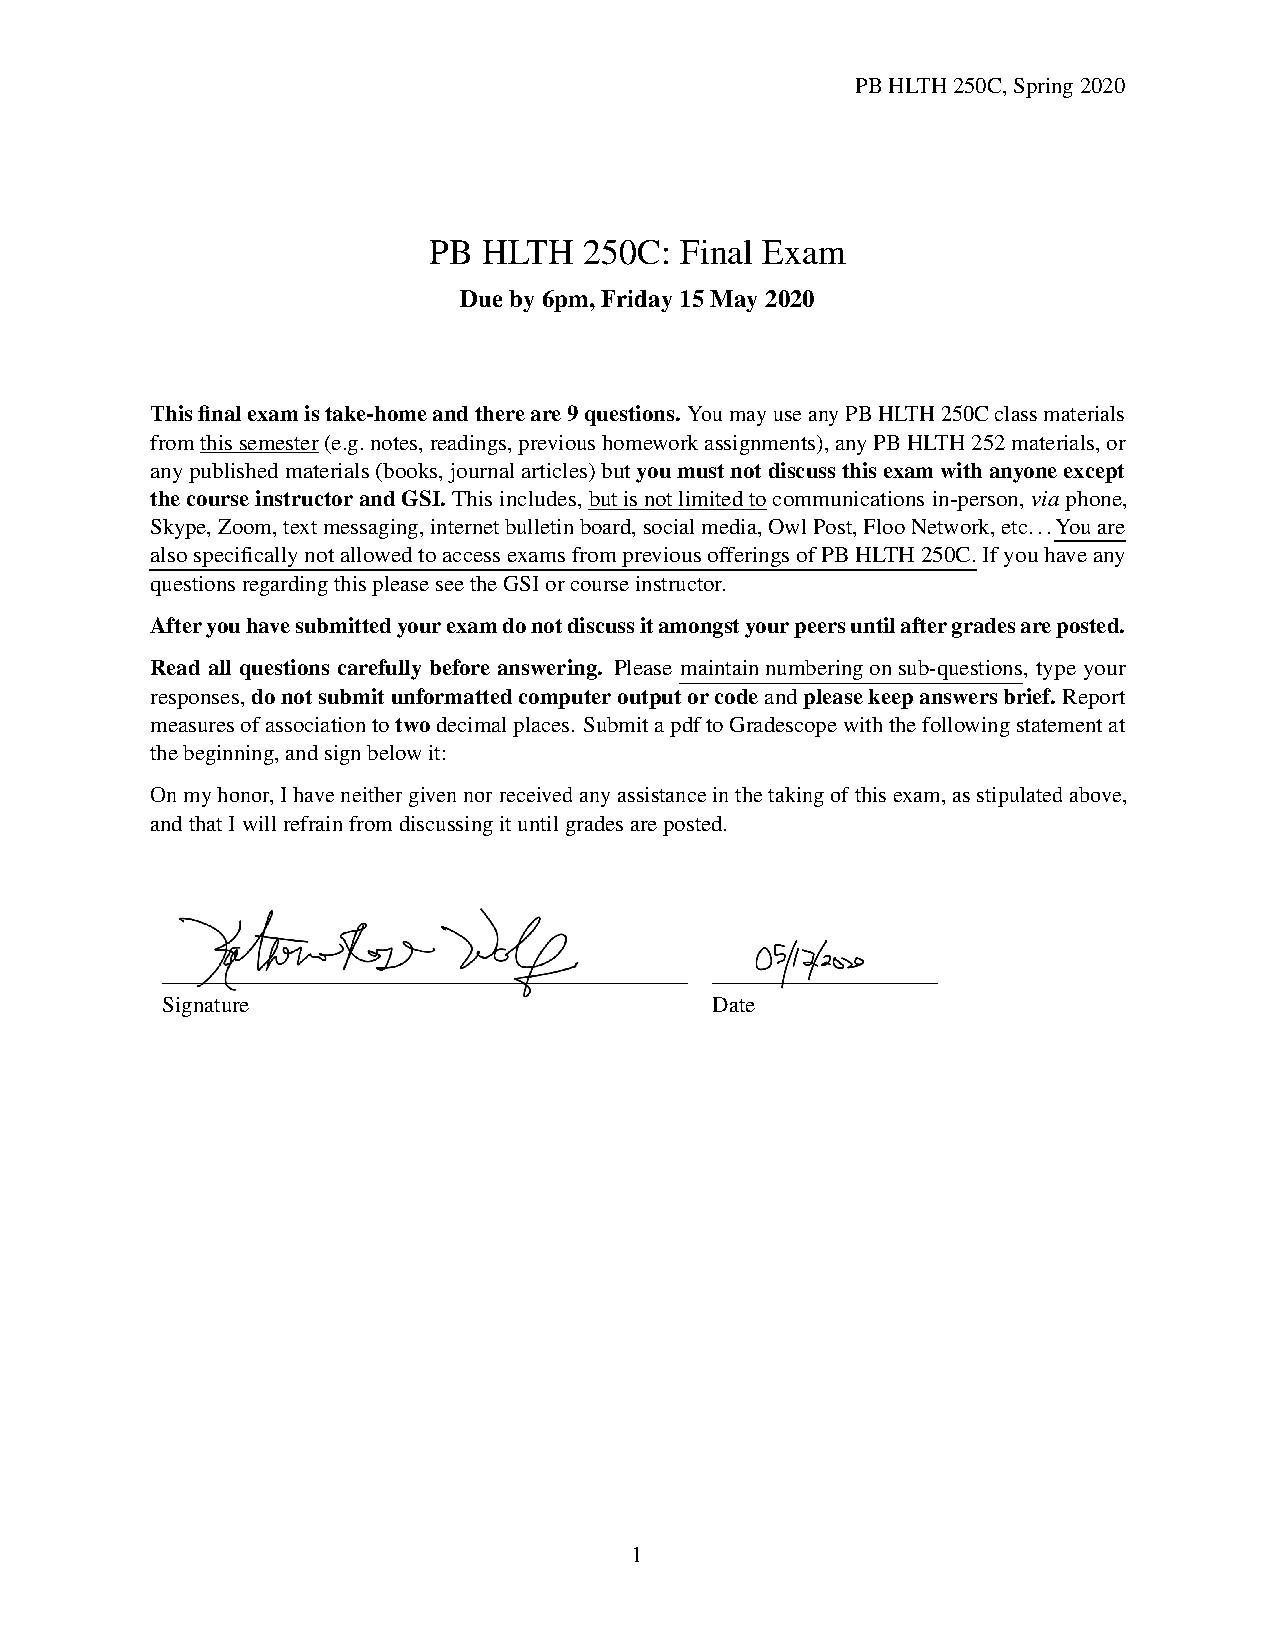
\includegraphics[height=6in]{signature_page}

\end{center}

\newpage

\begin{center}

\section{Questions}

\end{center}

\section{Bias analysis}

\textbf{Answer the following \textit{TRUE/FALSE} questions regarding bias analysis in general and \textit{provide a 1-2 sentence justification} (please read carefully). (5 points each)}

\begin{enumerate}[label=\textbf{\arabic*.}]
  \item \textbf{Deterministic bias analysis incorporates uncertainty in the bias parameters into your analysis.}

FALSE.

  \item \textbf{Probabilistic bias analysis yields a range of bias-corrected measures of association.}

TRUE.

  \item \textbf{The gamma distribution is a good choice for the distribution of the bias parameter for a proportion/prevalence/probability.}

  \item \textbf{The normal distribution is a good choice for the distribution of the bias parameter for a log-relative risk.}

  \item \textbf{One reason quantitative bias analysis is important is that systematic errors can be larger than random errors.}

TRUE.

\end{enumerate}

\newpage

\section{Paper evaluation}

\textbf{A paper by Keil et al. (2014) in \textit{Environmental Health} examined the association between exposure to imidacloprid (a common flea and tick medication for pets) and autisum spectrum disorder (ASD) among children. Read the accompanying paper, paying particular attention to the methods and results sections, and answer the following questions regarding the methodological approach and presentation of results \textit{(please keep answers brief)}:}

\begin{enumerate}[label=\textbf{\arabic*.}]\addtocounter{enumi}{5}
  \item \textbf{The authors mention using "3 jointly estimated models to simultaneously model the 'true' exposure and estimate its association with ASD." For the analysis in this paper, write out each of these models as described by the authors.\footnote{Note correction at top of page 3. Text should read: ’probability of reported exposure, given "true" exposure and case/control status...’} Consider only the non-differential misclassification scenario (group 2). Give definitions for each of the covariates and parameters in your models. Specify any distributional assumptions for the outcomes on the models, but here you do not need to specify the priors on the model parameters: \textit{Hint: refer to misclassification example from the Bayesian Bias Analysis lecture.}}
  \begin{enumerate}[label=\textbf{\alph*.}]
    \item \textbf{Exposure model (10 points)}
    \item \textbf{Measurement model (10 points)}
    \item \textbf{Outcome model (10 points)}
  \end{enumerate}


\newpage

  \item \textbf{The authors describe a sequence of analyses where each one treats the sensitivity and false positive rate (1-specificity) as fixed. In the case of non-differential misclassification (group 2), sensitivity ranges from 0.70-0.95 and false positive probability (1-specificity) from 0.00-0.20 for both cases (ASD) and controls (TD). Instead of specific fixed scenarios, describe one possible set of prior distributions for sensitivity and specificity that would be consistent with these ranges of values (5 points) \textit{Hint: Assume there is no prior probability outside of the stated ranges. You should specify two reasonable distributions of your choice (one for each bias parameter), and include specific values for the hyperparameters.}}
  
\newpage

  \item \textbf{The model above assumes non-differential exposure misclassification.}
  \begin{enumerate}[label=\alph*]
    \item \textbf{Modify and present the approopriate sub-model from question 6 to accommodate \textit{differential} misclassification (this will only involve one of (a), (b), or (c)). Make sure to define each of the necessary bias parameters in this new sub-model. (5 points)}
    \item \textbf{Assuming this modification, specify the necessary prior distributions for the bias parameters consistent with the group 3 scenario (see Figure 2). (5 points)}
  \end{enumerate}
\end{enumerate}

\newpage

\section{Analytic plan}

\begin{enumerate}\addtocounter{enumi}{8}

  \item \textbf{Given the analysis and methodological issue that you outlined on the midterm, \textit{briefly} outline an plan for the analysis. Consider writing this in the format you would for a MPH capstone proposal or dissertation prospectus. Be specific about 1) target parameter, 2) modeling forms, 3) covariates included, and 4) how you will inform any priors (e.g. for Bayesian analysis or probabilistic bias analysis). Include an expression for the model form (you can denote sets of covariates in vector notation for brevity). (30 points) LIMIT YOUR ANSWER TO ONE PAGE OR LESS.}

\end{enumerate}

\newpage

\hypertarget{bonus-3-points}{%
\section{Bonus (3 points)}\label{bonus-3-points}}

\textbf{Include (with your answers here) documentation that you have completed the online course evaluation for PBHLTH 250C. (And thank you!) (Please do not include any information on your
responses to the questions.)} \color{black}

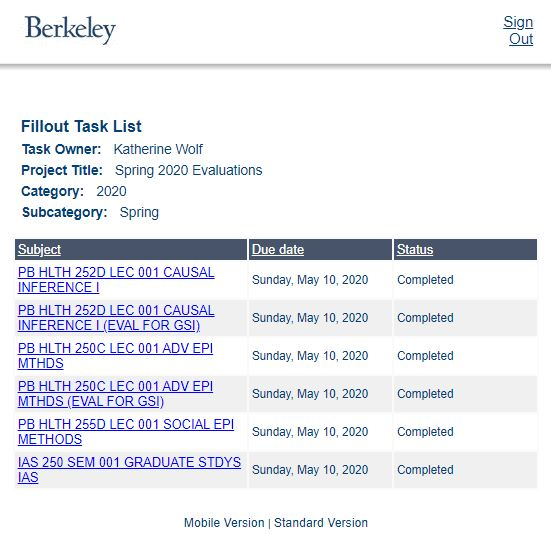
\includegraphics{course_evaluation.jpg}

\end{document}
